\documentclass{article}
\usepackage[utf8]{inputenc}
\usepackage[margin=1in]{geometry}
\usepackage{float}
\usepackage{tikz}
\usepackage{tikz-qtree}

\title{Data Structures: Problem Set 4}
\author{Jackie Luo}
\date{April 19, 2015}

\begin{document}
\maketitle

\section{Theory}

\subsection{}
a.
\newline
\begin{figure}[H]
\centering
\begin{tikzpicture}
\Tree [.3 ]
\end{tikzpicture}
\caption{[3]}
\end{figure}

\begin{figure}[H]
\centering
\begin{tikzpicture}
\Tree [.3 9 \edge[draw=none]; {} ]
\end{tikzpicture}
\caption{[3, 9]}
\end{figure}

\begin{figure}[H]
\centering
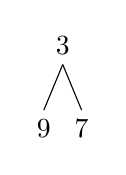
\begin{tikzpicture}
\Tree [.3 9 7 ]
\end{tikzpicture}
\caption{[3, 9, 7]}
\end{figure}

\begin{figure}[H]
\centering
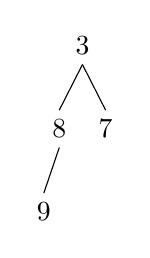
\begin{tikzpicture}
\Tree [.3 [.8 9 \edge[draw=none]; {} ] 7 ]
\end{tikzpicture}
\caption{[3, 8, 7, 9]}
\end{figure}

\begin{figure}[H]
\centering
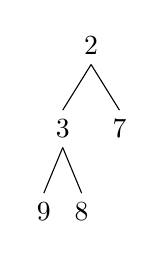
\begin{tikzpicture}
\Tree [.2 [.3 9 8 ] 7 ]
\end{tikzpicture}
\caption{[2, 3, 7, 9, 8]}
\end{figure}

\begin{figure}[H]
\centering
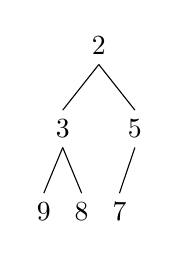
\begin{tikzpicture}
\Tree [.2 [.3 9 8 ] [.5 7 \edge[draw=none]; {} ] ]
\end{tikzpicture}
\caption{[2, 3, 5, 9, 8, 7]}
\end{figure}

\begin{figure}[H]
\centering
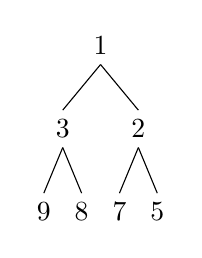
\begin{tikzpicture}
\Tree [.1 [.3 9 8 ] [.2 7 5 ] ]
\end{tikzpicture}
\caption{[1, 3, 2, 9, 8, 7, 5]}
\end{figure}

\begin{figure}[H]
\centering
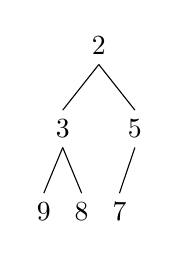
\begin{tikzpicture}
\Tree [.2 [.3 9 8 ] [.5 7 \edge[draw=none]; {} ] ]
\end{tikzpicture}
\caption{[2, 3, 5, 9, 8, 7]}
\end{figure}

\begin{figure}[H]
\centering
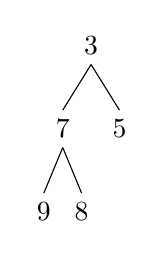
\begin{tikzpicture}
\Tree [.3 [.7 9 8 ] 5 ]
\end{tikzpicture}
\caption{[3, 7, 5, 9, 8]}
\end{figure}

\begin{figure}[H]
\centering
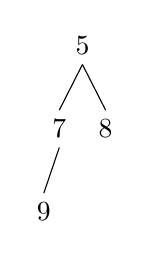
\begin{tikzpicture}
\Tree [.5 [.7 9 \edge[draw=none]; {} ] 8 ]
\end{tikzpicture}
\caption{[5, 7, 8, 9]}
\end{figure}

\noindent b.
\newline
Max Heap: [9, 8, 7, 3, 2, 5, 1]
\newline
1: [8, 3, 7, 1, 2, 5, 9]
\newline
2: [7, 3, 5, 1, 2, 8, 9]
\newline
3: [5, 3, 2, 1, 7, 8, 9]
\newline
4: [3, 1, 2, 5, 7, 8, 9]
\newline
5: [2, 1, 3, 5, 7, 8, 9]
\newline
6: [1, 2, 3, 5, 7, 8, 9]

\subsection{}
Here's a brief example that shows that QuickSort is unstable, as the two 32s change order in the sorting process, with 21 as the pivot:
\begin{table}[h]
\centering
\begin{tabular}{|l|l|l|l|l|l|l|l|}
\hline
$32_1$ & $32_2$ & 8 & 64 & 2 & 51 & 1 & 21 \\ \hline
1 & $32_2$ & 8 & 64 & 2 & 51 & $32_1$ & 21 \\ \hline
1 & 2 & 8 & 64 & $32_2$ & 51 & $32_1$ & 21 \\ \hline
1 & 2 & 8 & 21 & $32_2$ & 51 & $32_1$ & 64 \\ \hline
\end{tabular}
\end{table}

\subsection{}
Here's an example of the best-case running time of $\theta$(N) for Quick Select:
\newline
34, 8, 64, 2, 51, 36, 21, k = 5
\newline
The pivot using the median-of-threes strategy is 34, so $S_1$ consists of 8, 2, 21 (3) and $S_2$ consists of 64, 51, 36 (3). Since $k > S_1$, we know that the kth smallest element is in $S_2$.
\newline
64, 51, 36, k = 1
\newline
The pivot using the median-of-threes strategy is 51, so $S_1$ consists of 36 (1) and $S_2$ consists of 64 (1). Since $k \leq S_1$, we know that k is in $S_1$, and $S_1$ only contains the value 36, so 36 is the kth smallest element.


\end{document}